\documentclass[11pt, twoside]{report}
\usepackage[utf8]{inputenc}
\usepackage[english]{babel}
%\usepackage{times}
\usepackage{verbatim}
\usepackage[table,xcdraw]{xcolor}
\usepackage{microtype}
\usepackage{titlesec}
\usepackage{setspace} %table of contents spacing
\usepackage{epsfig}
\usepackage{subcaption}
%\usepackage{gensymb}
\usepackage{wrapfig}
\usepackage{array}
\usepackage{tocloft}
\renewcommand{\cftsecaftersnum}{.}
\usepackage{secdot}
\usepackage[colorlinks=true, linkcolor = black]{hyperref}
%\usepackage[usenames, dvipsnames]{color}
\usepackage{fancyhdr} %header
\usepackage[Lenny]{fncychap}
\usepackage[a4paper, portrait, margin = 1.3in]{geometry}
\usepackage[utf8]{inputenc} %For
\usepackage[T1]{fontenc}
\usepackage{amssymb} %for R of real number
\usepackage{amsmath}% for "n times"
\usepackage{makeidx} %making index


\pagestyle{fancy}
\fancyhf{}
\fancyhead[LE]{\textbf{\thepage}}
\fancyhead[RE]{\textbf{\nouppercase{\leftmark}}}
\fancyhead[RO]{\textbf{\nouppercase{\rightmark}}}
\fancyhead[LO]{\textbf{\thepage}}

\fancypagestyle{plain}{%
  \renewcommand{\headrulewidth}{0pt}%
  \fancyhf{}%
}


\usepackage{etoolbox}
\makeatletter
%\ patchcmd{<cmd>}{<search>}{<replace>}{<success>}{<failure>}
\patchcmd{\chaptermark}{\@chapapp\ }{}{}{}
\makeatother

\newcommand{\red}[1]{\textcolor{red}{#1}}
\newcommand{\blue}[1]{\textcolor{blue}{\textbf{figure: #1}}}
\newcommand{\teal}[1]{\textcolor{teal}{\textbf{equation: #1}}}
\newcommand{\purple}[3]{\textcolor{purple}{\textbf{\textit{#1}, #2, #3}}}

\begin{document}

%%%%%%%%%%%%%%%%%%%%%%
%%%%%%%%%%TITLE PAGE%%%%%%%
%%%%%%%%%%%%%%%%%%%%%%%
\begin{titlepage}
    \begin{center}
        \begin{figure}[hbt!]
             \centering
             
\includegraphics[width=0.3 \textwidth]{./figures/unimi_logo_tesi}
        \end{figure}
        \textbf{\Large{UNIVERSIT\`A DEGLI STUDI DI MILANO}}\\
        \vspace{12pt}
        \Large{FACOLT\`A DI SCIENZE E TECNOLOGIE}\\
        \Large{DIPARTIMENTO DI FISICA}\\
        \Large{Corso di Laurea triennale in Fisica (L-30)}
        \vspace{24pt}
        \hrule
        \vspace{24pt}
        \textbf{\Large{Quantum Walks with Time-Dependent Hamiltonians}\\ \large{and their application to the spatial search problem on graph}} \\

    \end{center}
    \vspace{120pt}
    \begin{flushleft}
        Relatore : \textbf{Prof. Matteo G.A. Paris}\\
        Correlatore: \textbf{Prof. Stefano Olivares}\\
        Correlatrice: \textbf{Dott.sa Claudia Benedetti}
    \end{flushleft}
    \vspace{12pt}
    \begin{flushright}
        Tesi di Laurea di:\\
        \textbf{Matteo Garbellini}\\
        Matricola 885615\\
        Anno Accademico 2019/2020
    \end{flushright}
    %\begin{flushright}
    %    Pacs: 98.65.-r
    %\end{flushright}
\end{titlepage}
\newpage

%%%%%%%%%%%%%%%%%%%%%%
%%%%%%%%%%ABSTRACT%%%%%%%
%%%%%%%%%%%%%%%%%%%%%%%
\newpage
\thispagestyle{empty}
\textbf{\Large{Abstract}} \\ \\
\noindent
In this thesis we study the properties of quantum walks with time dependent hamiltonian, focusing in particular on the application to the quantum search problem on graph. We compare the time independent and the time dependent approach for two graph topologies, the circular and the complete graph, which represent respectively the worst and best case scenario for the known quantum search. We also investigate the role of the function that regulates the time-dependance of the hamiltonian in the time scaling at which the solution is found. Lastly we exploit the consequences of the adiabatic theorem to study the localization properties of the time-dependent approach.

%%%%%%%%%%%%%%%%%%%%%%
%%%%%%%%%%TABLE OF CONTENTS%%%%%%%
%%%%%%%%%%%%%%%%%%%%%%%
\newpage
\thispagestyle{empty}
\doublespacing
\tableofcontents
\onehalfspacing

%%%%%%%%%%%%%%%%%%%%%%
%%%%%%%%%%LIST OF FIGURES%%%%%%%
%%%%%%%%%%%%%%%%%%%%%%%
\newpage
\thispagestyle{empty}
\listoffigures


%%%%%%%%%%%%%%%%%%%%%%
%%%%%%%%%%INTRODUCTION\textbf{%%%%%%%
%%%%%%%%%%%%%%%%%%%%%%%
\newpage
\chapter*{Introduction}
\addcontentsline{toc}{chapter}{Introduction}


%%%%%%%%%%%%%%%%%%%%%%
%%%%%%%%%%PRELIMINARIES%%%%%%%
%%%%%%%%%%%%%%%%%%%%%%%
\newpage
\thispagestyle{empty}
\chapter{Preliminaries}

\section{Graph Theory}
A graph G is defined as a ordered pair $(V,E)$, where V is a set of vertices and E is a set of edges, which represent the connection between any two pair of vertices. If indeed any two vertices $(i,j)$ are connected by an edge we define as adjacent, and from this we can construct the \textit{adjacency matrix} A as:
\begin{equation}
A_{ij} = \begin{cases} 1 & (i,j)\in G \\ 0 & \mbox{otherwise} \end{cases}
\end{equation}
which represents the connectivity of the graph. We can then describe the degree of each vertex of the graph, namely the number of vertices (excluding itself) connected to it, through the \textit{degree diagonal matrix} $D_{jj} = deg(j)$.\\
It is also useful to introduce the \textit{laplacian matrix} defined as
\begin{equation}
  L = A-D
\end{equation}
which we'll later see describes the quantum walk evolution.\\
In the quantum realm a vertex is a vector in an N dimensional Hilber space, so that a vertex $|j\rangle$ can be represented in the following way
\begin{equation}
  |j\rangle = \begin{pmatrix} 1 \\ 0 \\ 0 \\ .. \\0 \end{pmatrix}
\end{equation}

Throughout this work we focus our attention on two particular graph topologies: the \textbf{circular} graph and the \textbf{complete} graph (FIG. 1).


\begin{figure}[ht]
\centering
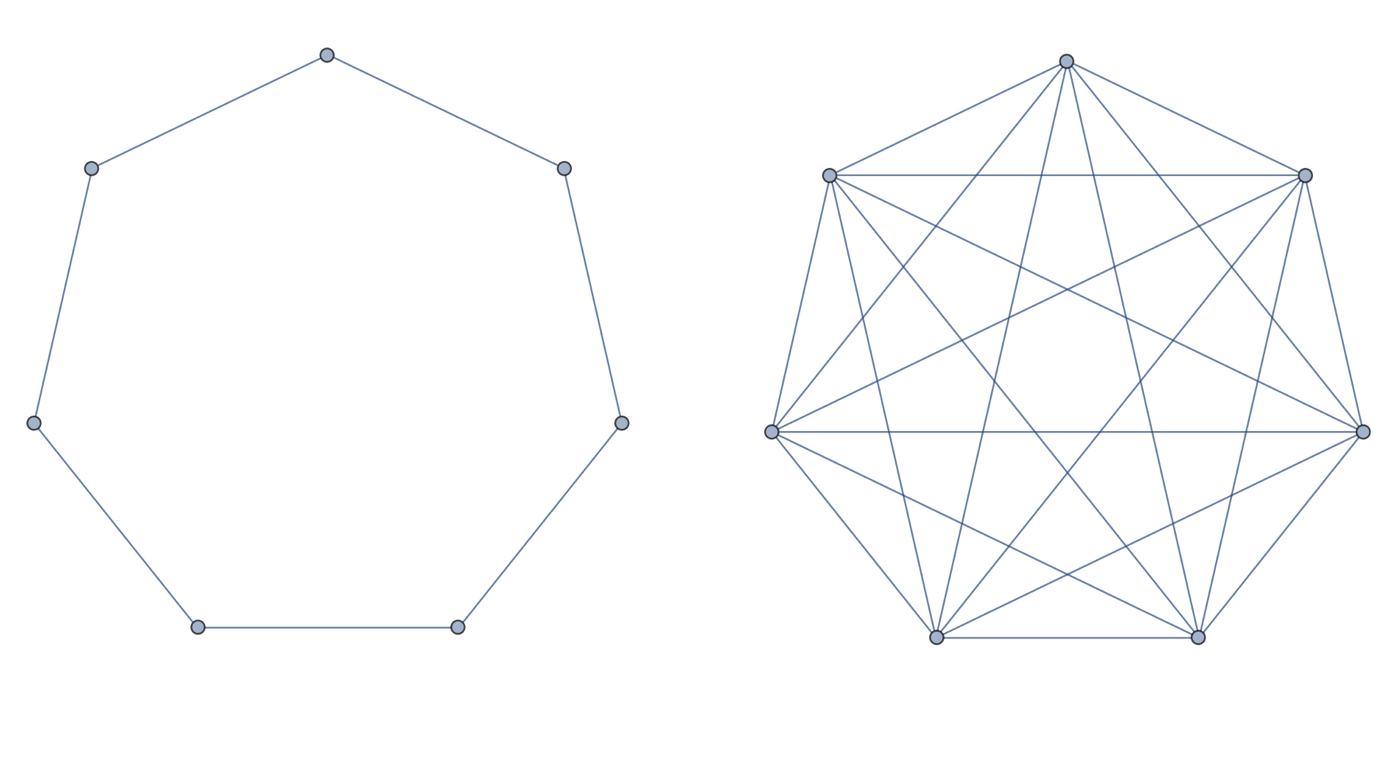
\includegraphics[width=9.5cm]{./figures/graph.png}%
\caption[Pictorial representation of circular and complete graph]{Pictorial representation of a circular graph (left) and a complete graph (right) with N=7}
\end{figure}

\section{Quantum Walks}
The continous time quantum walk is the direct analougue of the classical random walk. Given a graph G, a random walk is a Markov process with a fixed probability for unit time $\gamma$ of jumping to an adjacent vertex $j$. This particular walk can be described by a linear differential equation in terms of probability, namely

\begin{equation}
  \frac{d}{dt}p_j(t) = \gamma\sum_{k}L_{jk}p_k(t)
\end{equation}

where $p_j(t)$ is the probability of being on the vertex $j$ at time $t$.\\
The quantum analogue takes place in an N-dimentional Hilbert space spanned by the states (vertex) $|j\rangle$ of the graph G. Instead of considering the classical probability as we previosuly did, we consider the probability time-dependent amplitudes $q_j(t) = \langle j|\psi(t)\rangle$, where $|\psi\rangle$ is a general time-dependent state. The differential equation takes thus the form of

\begin{equation}
  i\frac{d}{dt}q_j(t) = \sum_{k}H_{jk}q_k(t)
\end{equation}
The continous-time quantum walk is defined by letting $H=-\gamma L$, where $L$ is the previosuly defined Laplacian matrix.

\section{Grover's Quantum Search}
\red{This section should include the standard Grover's Quantum Search to give the contex for the quantum walk approach.}

\section{Quantum Search with Continous-Time Quantum Walk}
\purple{Spatial Search by Quantum Walk}{A. Childs, J. Goldstone}{quant-ph/0306054v2}\\
We now address the quantum search problem firstly formulated as Grover's algorithm and then extending it to the search on a graph using quantum walks. \\
To approach the Grover problem with quantum walk it's necessary to modify the hamiltonian such that the vertex $|w\rangle$, i.e. the target, is somewhat special. Following Grover's oracle an oracle hamiltonian $H_w$ is introduced

\begin{equation}
  H_w = -|w\rangle\langle w|
\end{equation}

which in particular has energy zero for all but the vertex $|w\rangle$ for which it has enenergy $-1$. Therefore the Grover problem, i.e. quantum search, becomes finding the ground state of such hamiltonian. To do so we consider the time-independent hamiltonian of the form
\begin{equation}
  H = -\gamma L + H_w = -\gamma L -|w\rangle\langle w|
\end{equation}
where L is the laplacian of the graph, which contains the information of the dynamics over that particular graph topology. The evolution of the quantum walk is therefore governed by this hamiltonian.\\

The quantum search routine works as follow:
\begin{itemize}
  \item we consider the superposition of all possible states, namely
  \begin{equation}
    |s\rangle = \frac{1}{\sqrt{N}}\sum_j|j\rangle
  \end{equation}

  \item we find the evolved state using the hamiltonian for a time T $H$
  \begin{equation}
  |\psi(T)\rangle = U(T)|s\rangle  = \mbox{exp}\Big\{-\frac{i}{\hbar}HT\big\}|s\rangle
  \end{equation}
  (Note that this evolution is valid only for time-independent hamiltonians.)

  \item we then measure the state onto the target $|w\rangle$ and find the corrisponding probability
  \begin{equation}
    p = |\langle w|\psi(T)\rangle|^2
  \end{equation}

\end{itemize}

The objective is to find the optimal value of $\gamma$ so that the probability of the system of finding itself in $|w\rangle$ is as close as possible to 1 for the smallest T.

\subsection{Search on Complete Graph}
We now look at the search on a complete graph. This case is particularly interesting since it can be solved analitically\\
\red{to be continued}

\section{Adiabatic Theorem}
\purple{Quantum Computation by Adiabatic Evolution}{E. Farhi, J. Goldstone, S. Gutmann, M. Sipser}{quant-ph/0001106}\\


A quantum system evolves according to the Schroedinger equation
\begin{equation}
    i\frac{d}{dt}|\psi(t)\rangle = H(t)|\psi(t)\rangle
\end{equation}
and defining the instantaneous eigenstates and eigenvalues of H(t) by
\begin{equation}
    H(t)|l;t\rangle = E_l(t)|l;t\rangle
\end{equation}
such that $E_0(t) \geq E_1(t) \geq ... \geq E_{N-1}(t)$. \\
The adiabatic theorem states that if the gap between the two lowest energy levels, $E_{1}(t) - E_{0}(t) > 0$, is stritcly greater than zero then for $T\rightarrow \infty$ the probability of being in the ground state is equal to one, namely
\begin{equation}
    \lim_{T \to \infty} |\langle l=0;t = T | \psi(T)\rangle| = 1
\end{equation}
This means that if the system is chosen to evolve at a slow enough rate, the instantaneous hamiltonian will remain in the ground state throught the evolution. It is useful to consider a smooth one-parameter hamiltonian $H(s)$ such that $s=t/T$, with $t \in [0,T]$ so that $s \in [0,1]$.
Let's now define the energy minimum gap by
\begin{equation}
    g_{min} = \min_{0 \leq s \leq 1} (E_1(s)-E_0(s))
\end{equation}
In addition we can find a time lower bound $T^*$ such that for $T\gg T^{*}$ the probability is arbitrarily close to 1, in detail
\begin{equation}
    T \gg \frac{\varepsilon}{g^{2}_{min}}
\end{equation}
where
\begin{equation}
    \varepsilon = \max_{0 \leq s \leq 1} \Big| \Big\langle l=1;s\Big| \frac{dH(s)}{dt} \Big| l=0;s\Big\rangle\Big|
\end{equation}

\subsection{Computation by Adiabatic Evolution}
Let's now discuss how to take advantage of the adiabatic theorem introducting the usual way in which the adiabatic evolution is implemented. It is often presented a problem hamiltonian $H_P$ whose ground state is not so straight forward to find; on the other hand we can prepare the system in abeginning hamiltonian $H_B$ whose ground state is known. The problem hamiltonian encodes the solution of the problem, while the beginning hamiltonian is a tool for easily preparing the state to be evolved. The adiabatic implementation then consists, assuming that the ground state of $H_P$ is unique, in having a time dependent hamiltonian $H(s)$ such that
\begin{equation}
    H(s) = (1-s)H_B + s H_P
\end{equation}
In this way we can prepare for $s=0$ the system in $H_B$ and let it evolve so that for $s=1$ it reaches $H_P$. Thanks to the adiabatic theorem, if it's made to evolve sufficiently slowly we will find ourself in the ground state of the problem hamiltonian, which is exactly the solution.



%%%%%%%%%%%%%%%%%%%%%%
%%%%%%%%%%QUANTUM WALKS WITH TIME DEPENDENT HAMILTONIANS%%%%%%%
%%%%%%%%%%%%%%%%%%%%%%%
\newpage
\thispagestyle{empty}
\chapter{Quantum Walks with Time-Dependent Hamiltonians}
We now turn our attentiont to a time-dependent implementation of the hamiltonian governing the evolution of the quantum walks. In particular we look at the application of such QW to the search problem on two selected graph topology, the complete and the circular graph. These two represent respectively the best and worst case scenario, namely the complete graph is known to work with the time-independent implementation \cite{Childs2004} and the local adiabatic evolution \cite{Roland2002} from which we constructed our work.

\section{Search with Time-Dependent Hamiltonian}
Following the adiabati evolution discussed in the preliminaries, we consider a search hamiltonian consisting in an oracle term and a laplacian term, such that at the beginning of the evolution we hamiltonian is equal to the laplacian, while at the end it's equal to the oracle hamiltonian. Such hamiltonian is constructed in the following way:
  \begin{equation}
    H = (1-s(t))L - s(t)\beta|w\rangle\langle w|
  \end{equation}
where $|w\rangle$ represents the target of the search.
The function $s(t)$ (referred as \textit{step function}) regulates the evolution of the hamiltonian an plays a  crucial role in the final search probability, as we will later see. It is defined in the following way
  \begin{equation}
    s: [0,T] \rightarrow [0,1]
  \end{equation}
where T is the time at which the solution is found (or actually, the time that the system is made to evolve. A solution might not be found at such time, or at least found with low probability).



\subsection{Complete Graph}
\textbf{Note}: for this particular application is necessary to review some literature, in particular look at the work by Wong \& Meyer \cite{Wong2016}, where they studied the irreconcilable difference between quantum walks and adiabatic computation in the context of quantum search. they looked at the complete graph (or unstructured search) and showed that, even if the quantum walks approach and the adiabatic approach do work on their own, if made to evolve on the same path the usual structure of the Grover's oracle is not enough, and additional hamiltonian might be necessary. Further studies could be conducted using Farhi et al. different paths hamiltonian \cite{Farhi2002}.

\subsection{Circular Graph}
We now consider the case of the circular graph, for which we know that the time-independent quantum walk approach does not lead to significant results. Infact, we will use precisely those results as benchmarks for the time-dependent approach.\\
The hamiltonian that governs the quantum walks does not however presents any particular proprerties, to the point that the evolution of the initial state can't be derived analitically (or maybe not yet) and thus the process of finding such state has two follow different paths. \\
The time evolution operator follows from the time-ordering approach, namely:
  \begin{equation}
    S(t,t_0) = T exp \frac{1}{i\hbar}\Big\{ \int_{t_0}^{t} dt' H(t')\Big\}
  \end{equation}
where T is the time-ordering.

\noindent
In order to find the evolved state we can proceed in the following ways:
\begin{itemize}
  \item \textbf{Dyson Series}
  \item \textbf{Magnus Expansion}
  \item \textbf{Solve the Schroedinger differential equation}
\end{itemize}
Since we're only interested in finding the evolved state, having the exact form of the evolution operator is somewhat irrelevant. Focusing our attention on the solution of the differential equations also helps us from a computational point of view; indeed the implementation of the differential equation solver is much simpler than any of the other two possibilities.

\subsubsection*{Solving the Schroedinger Equation}
From the intial state $|\psi\rangle$ we're intested in finding the evolved state $|\psi(t)\rangle$, and we proceed solving the differential Schroedinger equation:
  \begin{equation}
    i\frac{d}{dt}|\psi(t)\rangle = H |\psi(t)\rangle
  \end{equation}
Since H is a matrix we had to solve it for components. Recalling that $|\psi\rangle$ is a vector in an N-dimensional Hilbert space, we need to solve N-differential equations of the form:

  \begin{equation}
  \frac{d}{dt}|\psi_i(t)\rangle = \sum_jH_{ij}|\psi_i(t)\rangle
  \end{equation}
We also need to impose boundary conditions, namely that $|\psi(0)\rangle = |\psi\rangle$, our initial ground state.

\subsection{Comments on the shape of s(t)}
As we mentioned previously the step function s(t) plays a crucial role in the evolution of the system. The classical adiabatic evolution by Farhi et al. \cite{Farhi2000} consists in a linear step function s(t) defined as $s(t) = \frac{t}{T}$, such that the systems evolves linearly. \\


We however investigate which is the optimal shape of s(t) for otpimal probability. We first consider, somewhat naively, the square root and the cubic root of t/T, and the square and third power of t/T. However, for the complete graph Ronald \& Cerf propose that the optimal shape of s(t) comes from considerations on the separation of the first two eigenvalues \cite{Roland2002}; in particular s(t) should be steeper for larger separation and flatter for small eigenvalues separation. This in indeed somewhat to be expected, considering that for the adiabatic theorem to hold the adiabatic time needs to have a certain value which dependes directly from the eigenvalues separation. \\
Following that approach we consider a similar step function that tries to emulate the one from Ronald \& Cerf. For this paricular reason we will refer to this particular step function as the Ronald-Cerf s(t) even though it's not exacly the same one they derived. \\


Follows here a summary of all the step functions considered in the analysis of the circular graph. Note that for the complete graph, since the solution is derived analitically such different s(t) are not considered nor of particular interest.
  \begin{itemize}
    \item \textbf{lin}: $s(t) = \frac{t}{T}$
    \item \textbf{sqrt}: $s(t) = \sqrt{\frac{t}{T}}$
    \item \textbf{cbrt}: $s(t) = \sqrt{\frac{t}{T}}$
    \item \textbf{Ronald-Cerf(k)}: $s(t) = \frac{1}{2}(2(x-1)^{k}+1)^2$
  \end{itemize}
For the Ronald-Cerf step function we considered different values of odd-k, $k=3,5,7$. It is clear that we need to include a picture of the different functions considered and the eigenvalues separation picture for a particular case.


\section{Results for the circular graph}
We now presents the results for the circular graph topology. As we mentioned before we're particularly interested in this topology since it's known to not work with the standard time-independent quantum walk approach, thus it can benefit the most from the time-dependent implementation. We will start describing the two possible results, namely the \textbf{search} and the \textbf{localization}, followed by some time-independent benchmarks and the time-dependent results. To compare the two approaches we introduce a quantity, the $\min\Big(\frac{T}{p}\Big)$ that describes the best combination of time and probability. We shall than make some considerations, in particular on the $\gamma$ (or $\beta$) parameter and the lower bound on time that is necessary to consider.

\subsection{Search vs Localization}
It is necessary to characterize two type of results, the \textbf{search} and the \textbf{localization}, which help us determine whether the time-dependent approach is somewhat superior to the time-independent approach.
  \begin{itemize}
    \item the (optimized) \textbf{search} describes the usual search, namely the finding of the solution with high probability (possibly unitary) for the smallest time as possible. As we shall see later, we also include the possibility of repeating the experiments an n-amount of time, splitting the probability by $1/n$; this clearly is not the same as a single iterations with unitary probability. Further discussions are due in the next sections.
    \item the \textbf{localization} on the other hand describes the finding of the solution with high probablity (and with the consequences of the adiabatic theorem we could easily say with almost unitary probability) without the need to optimize the time. This routine is clearly without interest in the case the optimized search does indeed work, but as we shall later see for the circular graph this is not the case and provides a successfull way to locate (hence, localization) a defects or similar.
  \end{itemize}

\subsection{Time-Independent Benchmark}
The first step of the analysis is to compute time-independent benchmarks. We computed the probability over a time-beta grid, with $T\in[0,N]$ and $\beta\in[0,2.5]$, where N is the dimension of the graph considered. An initial run of the probability distribution showed that \textit{it is worse than linear in T}, thus the need to see times greater than $T=N$ proved to be unnecessary. In addition Grover algorithm for the unstructured search (and the complete graph) goes like $\sqrt{N}$ and the adiabatic (globally, not locally) goes like $N$, thus focusing on $T \leq N$ made much more sense. \textbf{It's interesting to show a figure with the probability distribution for some sampled $\beta$ even for large time, giving the idea that the probability does indeed not increase with time and we can focus the attention to smaller T (T<N)}.
Throughout the analysis we will consider graphs up to N = 71, with only odd dimensions which makes a easier oracle placement (hamiltonian is somewhat symmetric). Additional considerations and reasoning for the time-beta grid can be found in Appendix A. \\


To display the results in an intuitive way we used a heatmap plot, which gives a good idea on the probability distribution for varying combinations of $(T,\beta)$:

  \begin{figure}[ht]
    \centering
    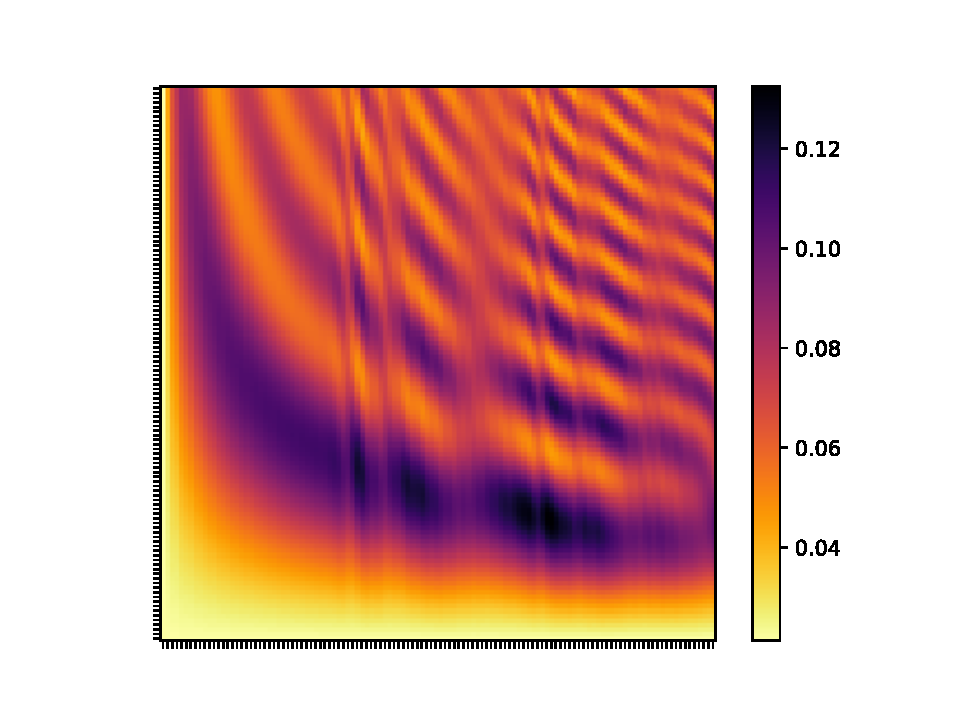
\includegraphics[width=9cm]{./figures/time_independent_benchmark_47}%
    \caption[Probability heatmap plot for the time-independent hamiltonian, N=47]{\textbf{Probability heatmap plot for the time-independent hamiltonian.} The figure shows the probability distribution for a circular graph of N=47 simulated using the time-independent hamiltonian, providing thus the necessary benchmark. Note that darker color do not represent probabilities close to one, but only higher probability regions.}
  \end{figure}

\subsubsection*{Comments on the probability distribution}
It is quickly noticeable that the probability distribution is not smooth, indeed it shows peaks (darker regions) and valleys (lighter regions). This is both present for fixed $\beta$, i.e. any orizontal line, and for fixed time, i.e. any vertical section considered. We will later see that this is somewhat a weakness of the time-independent approach, since a small variation of the parameter $\beta$, which reperesents as previosly mentioned the deepness of the well or an energy parameter, leads to possibly great variation of the probability. We shall call this fenomena \textbf{non-robustness}.

\subsection{Time-Dependent Results}
Similarly we computed the grid probability using the time-dependent hamiltonian previously introduced. To easily comparing the two methods we opted to consider the same time $T=N$, and from an initial run we discovered that the $\gamma$ parameter affected similarly the probability, namely the probability tended to be higher for smaller values of $\gamma$, thus we used approximately the same range. \\

The simulation is then run for all the step functions $s(t)$ previsouly discussed, and an intuitive heatmap plot is outputted.
\begin{figure}[ht]
\centering
\begin{tabular}{cc}
  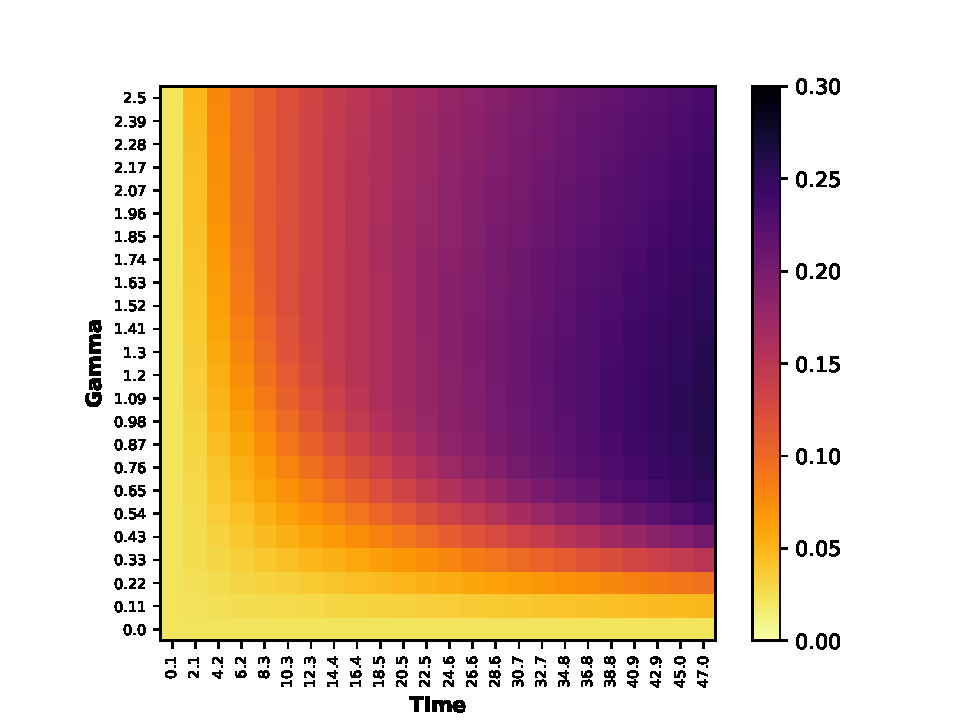
\includegraphics[width=75mm]{./figures/time_dependent_heatmap/47_heatmap_time_dependent_lin.pdf} &   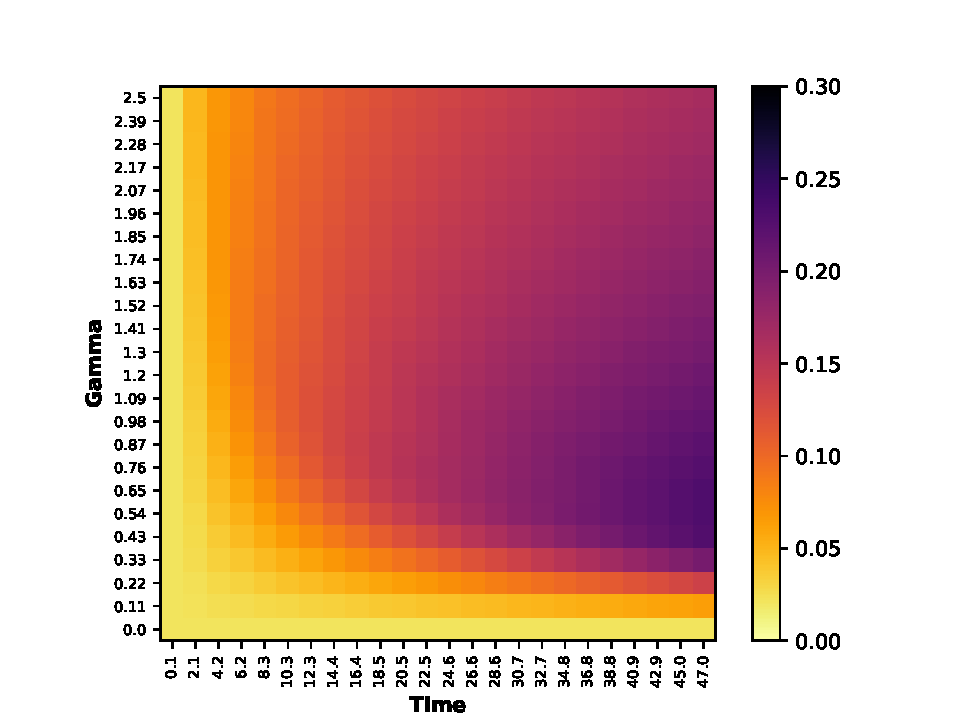
\includegraphics[width=75mm]{./figures/time_dependent_heatmap/47_heatmap_time_dependent_sqrt.pdf} \\
(a) lin & (b) sqrt\\[6pt]
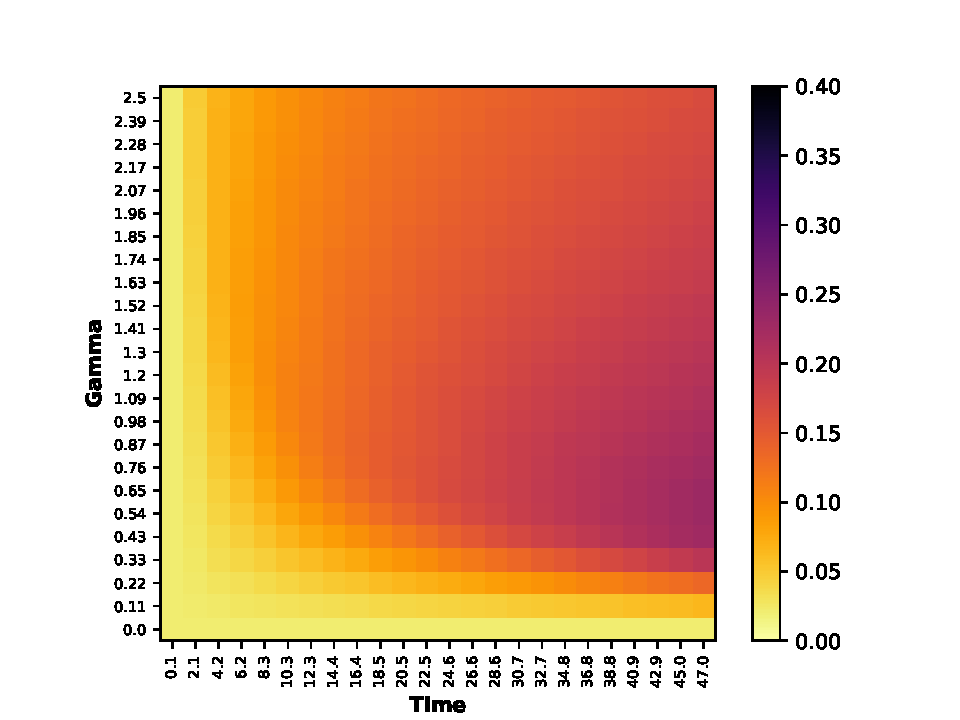
\includegraphics[width=75mm]{./figures/time_dependent_heatmap/47_heatmap_time_dependent_cbrt.pdf} &   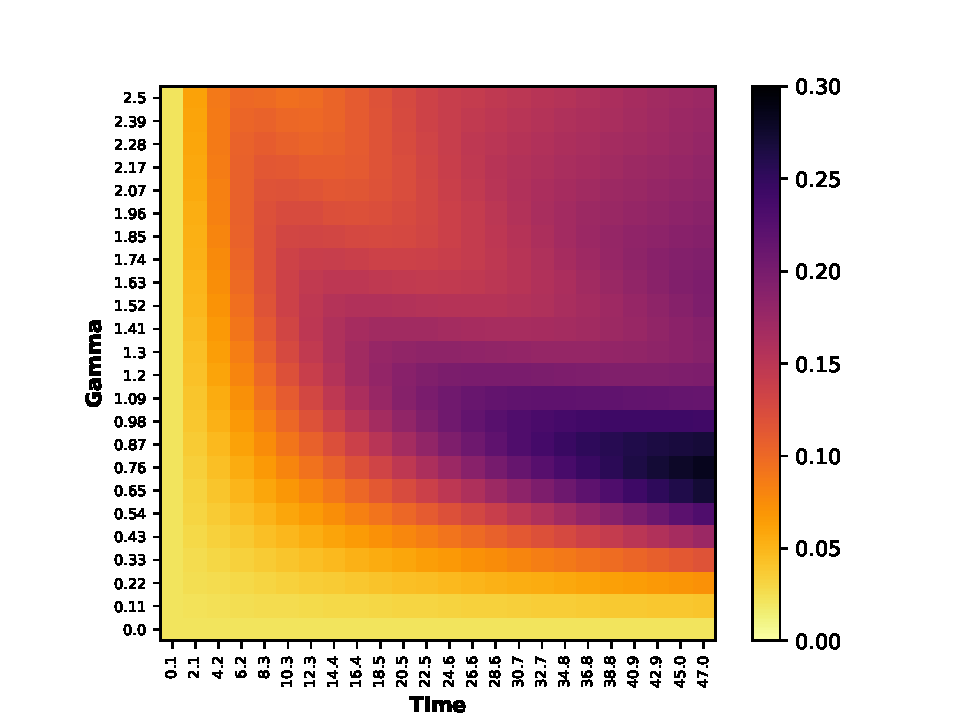
\includegraphics[width=75mm]{./figures/time_dependent_heatmap/47_heatmap_time_dependent_cerf.pdf} \\
(c) cbrt & (d) cerf\\[6pt]
\end{tabular}
\caption[Probability heatmap plot for the time-dependent hamiltonian, for different shapes of s(t)]{\textbf{Probability heatmap plot for the time-dependent hamiltonian, for different shapes of s(t).} The figure shows the probability distribution for a circular graph of N=47 evaluated using the time-dependent hamiltonian using the following step functions (a) linear, (b) $\sqrt{t/T}$, (c) $\sqrt[3]{t/T}$ and (d) Ronald-Cerf(3). Note that the probability gradient is normalized to p=0.3 to accentuate the difference in probability between different regions. }
\end{figure}

\subsubsection*{Comments on the probability distribution}
\subsection{Comparing the two approaches}
In order to compare the time-independent and time-dependent approaches it is necessary to consider a quantity that is somewhat meaningfull. Ww shall also differentiate between search and localization. We'll start discussing the latter.

\subsubsection*{Localization}
According to the adiabatic theorem discussed in the preliminaries, theoretically for large enough $T$ we should get a probability close to 1. The adiabatic theorem also provides a lower bound of time (that we shall call \textit{adiabatic time}) so that any $T$ much larger than that particular $T^*$. \\
As showed in Figure ? the time-independent approach does not produce higher probabilities for larger $T$, and thus not show any localization properties. On the othe hand the time-dependent one does indeed excels in the localization, as we can see in the following plot where the probability was evaluated up to large $T$ and for some sampled $\gamma$.

\begin{figure}[!ht]
    \centering
    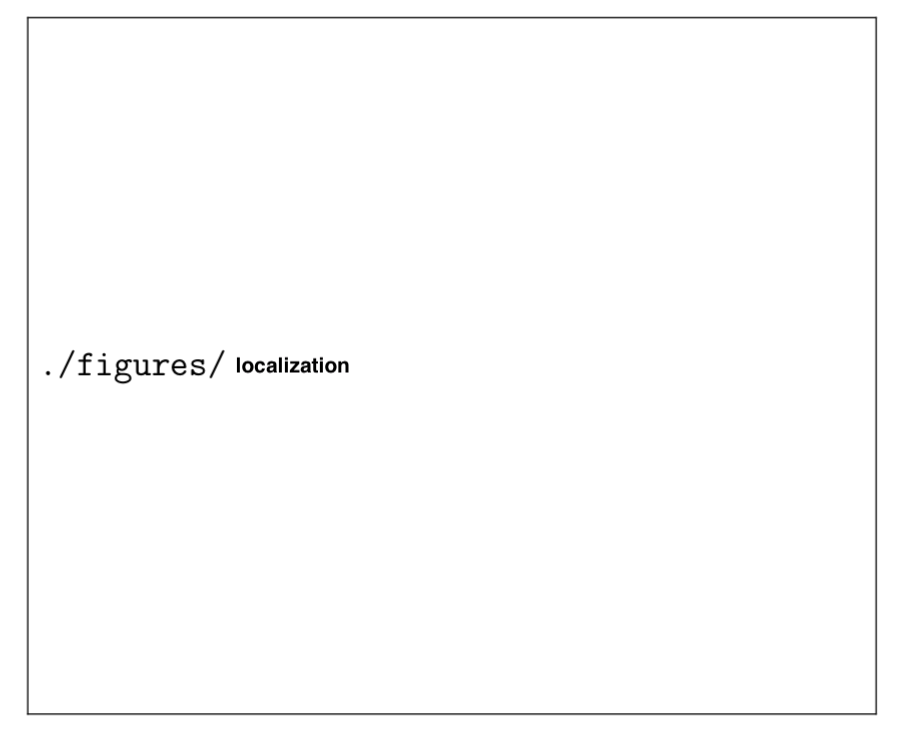
\includegraphics[width=9cm]{./figures/localization}%
    \caption[Probability distribution for large T showing localization properties]{\textbf{Probability distribution for large T showing localization property of the time-dependent approach.} The figure shows the probability distribution for a circular graph of N=47 evaluated using the time-dependent hamiltonian for large $T$ and sampled $\gamma$. The vertical line represents the \textit{adiabatic time}. It is thus clear that for large enough $T$ the probability converges regardless of the $\gamma$ parameter.}
\end{figure}

It is indeed clear from the picture above that for large enough $T$ the probability converges to unity. The role that the parameter $\gamma$ plays in this particular scenario is somewhat of lesser interest, since the probability goes to one (almost) regardless of the value of $\gamma$; it is however clear that different values of such parameter produce quite different values of $T$ at which the probability is equal to one. \\
The question is now indeed at what time does the probability goes to one? Can we extrapolate some kind of trend? and how influential is the $\gamma$ parameter? \textbf{This is still an open question that we should definitely address. And at first glance this localization property of the time-dependent hamiltonian is a great result: being almost independent on the $\gamma$ parameter means that the solution is always found. This is also particularly interesting for the complete graph, which works only for a specific value of $\gamma$ with the time-independent approach.}

\subsubsection*{Search}
In order to compare the two approaches for the so-called \textit{search} it is clear that we cannot simply consider the time at which the solution is found with unitary probability. We thus introduce a new quantity, namely:
  \begin{equation}
    \min\Big(\frac{T}{p}\Big)
  \end{equation}
What does this approach mean? \\
Since for the search we're interested in optimizing the time as well, finding the combination of $\gamma-T$ for which the probability is unitary does not provide any interesting insight. Additionally we've seen that the time-independent approach does not get to unitary probability for large T. It is thus necessary to consider a different approach, namely repeating the \textit{experiment} multiple times. If the combination $\gamma-T$ produces a probability $p<1$, statistically after $1/p$ run of the experiment we should get the correct result. The minimum of $1/p$ produces the smallest number of iterations necessary to get to unitary probability, and combining it with the time should give us the combination of time and probability such that the probability is unitary for the smallest time possible.\\


It is necessary to make additional considerations, in particular on the ration $T/p$. Recalling that we're dealing with a grid-evaluated probability, we know that the time $T$ varies linearly. On the other hand, as we can see with the following plot the probability does not increase linearly and thus the quantity $T/p$ (in this case for sampled $\gamma$) is far from a straight line (or as we would have hoped, any distribution that stood under the I quadrant bisector).

\begin{figure}[!ht]
\centering
\begin{tabular}{cc}
  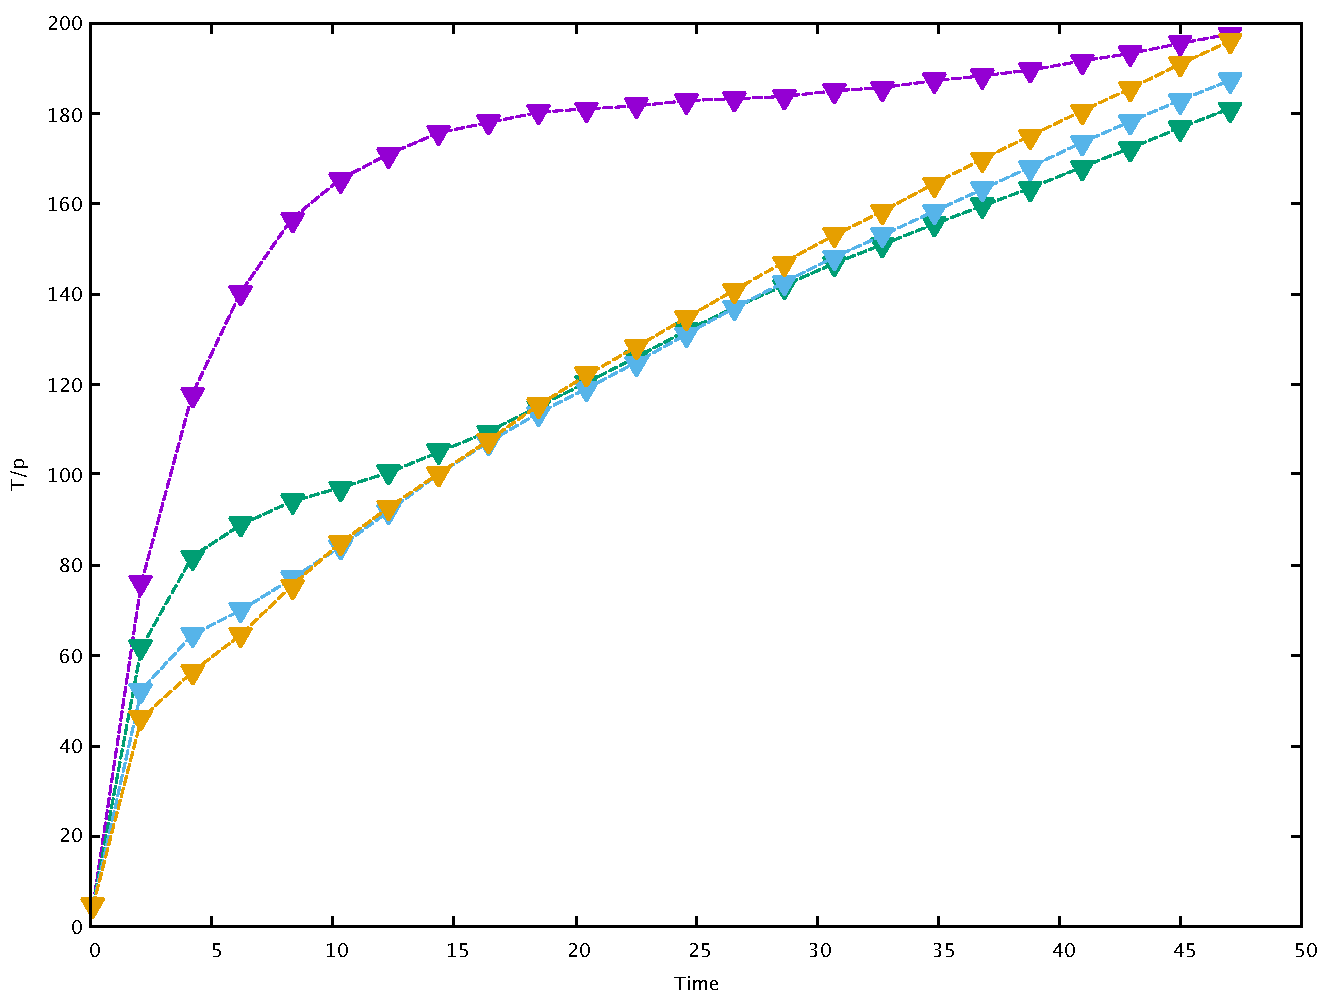
\includegraphics[width=75mm]{./figures/sampled_t_over_p/T_p_lin.pdf} &   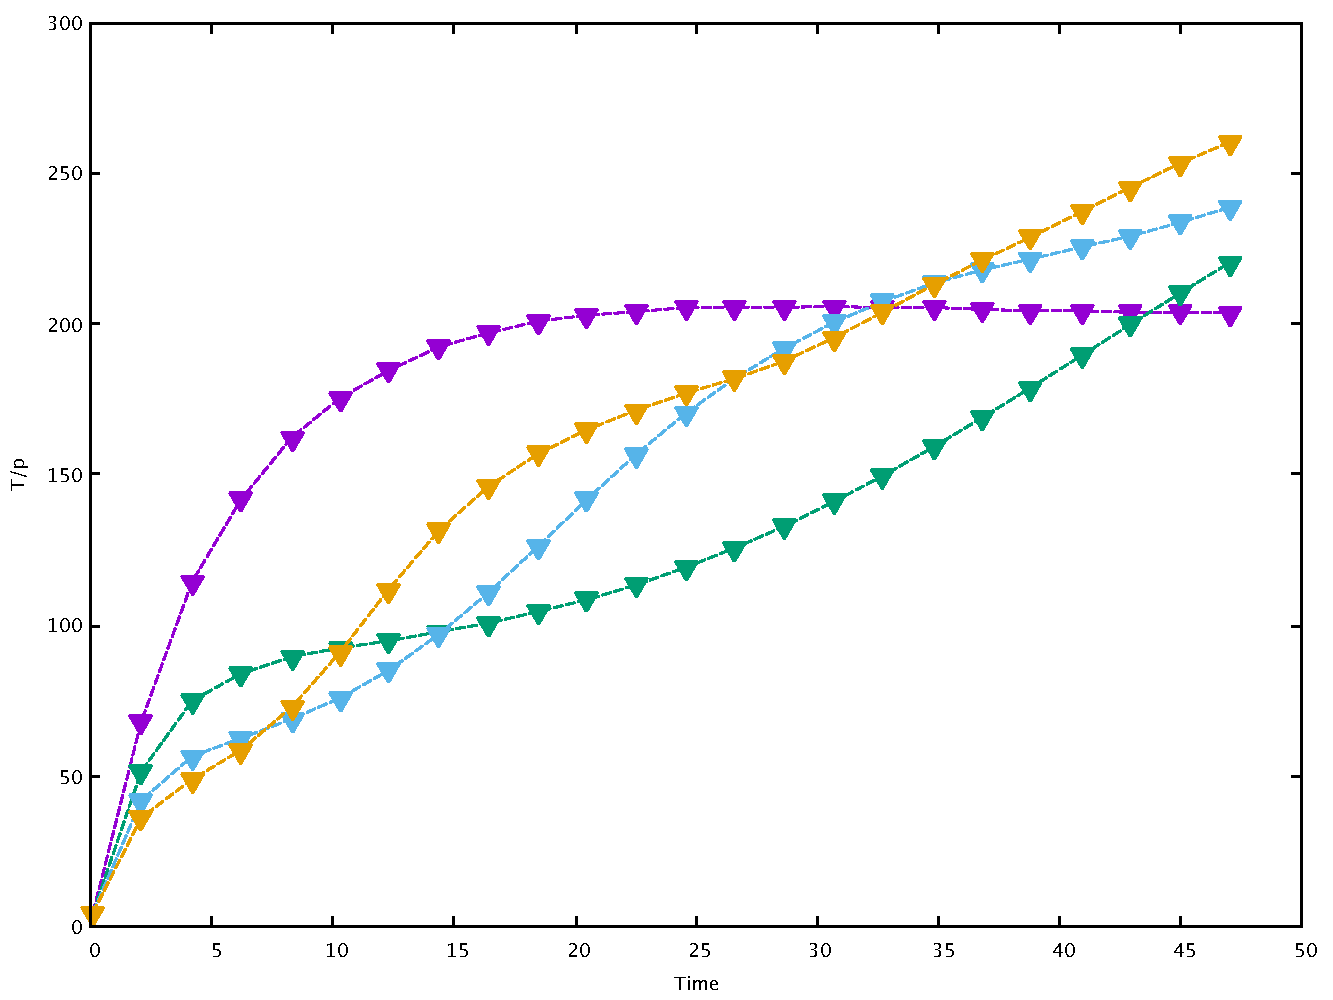
\includegraphics[width=75mm]{./figures/sampled_t_over_p/T_p_cerf.pdf} \\
(a) lin & (b) Ronald-Cerf\\[6pt]
\end{tabular}
\caption[Sampled T/p ]{\textbf{Sampled T/p to show that the min(T/p) will always be the smallest T available.}}
\end{figure}

 \textbf{How does this pose a problem?} The great issue with the quantity $T/p$ is that its minimum will always be found for the smallest time possible, regardless of the fact that for larger time, the probability of a single iteration could be higher.




%%%%%%%%%%%%%%%%%%%%%%
%%%%%%%%%%CONCLUSIONS%%%%%%%
%%%%%%%%%%%%%%%%%%%%%%%
\newpage
\chapter*{Conclusions}
\addcontentsline{toc}{chapter}{Conclusions}

%%%%%%%%%%%%%%%%%%%%%%{}
%%%%%%%%%%APPENDIX%%%%%%%
%%%%%%%%%%%%%%%%%%%%%%%
\newpage
\chapter*{Appendices}
\addcontentsline{toc}{chapter}{Appendices}
\phantomsection
\section*{Appendix A: Probability Grid Evaluation}
\addcontentsline{toc}{section}{Appendix A: Probability Grid Evaluation}
\phantomsection
\section*{Appendix B: Computational Routines}
In this section an overview of the computational methods is presented, focusing the attention on the \textbf{optimization algorithm} and the \textbf{differential equation solver}. Additionally the normalization error is discussed. Lastly computational reasoning for the \textbf{probability grid evaluation} are presented. \\

Most all numerical simulations were performed using \textbf{Python}. Numerical methods such as optimization and ODE Solver come directly from python's native \textbf{Scipy}. In addition, a CPU-multiprocessing library, \textbf{Ray}, has been used to speed up the grid probability evaluation quite noticeably. Heatmap plots were created using python matplotlib, while additional plots were created with gnuplot.

\subsection{Optimization Algorithm}
In Section III a series of benchmark were performed to compare the time-dependent and time independent hamiltonian approach to the search problem. In order to determine which optimization algorithm fitted the best for the task, a number of possible algorithm were tested, such as \textit{shgo, dualannealing, minimize, LHSBH} and \textit{Basin-Hopping}.\\ \\
Due to the oscillating nature of the probability (\red{a figure is needed}) the scipy native \textbf{Basinhopping algorithm} was used. As the name suggests the algorithm performs a series of randomized hops, i.e. jumps, of the coordinates in order to find the true maximum This fits particularly well with the series of maxima and minima of the probability function (for fixed $\gamma$) in the time-independent hamiltonian. \\\red{Additional information on the parameter used are needed (e.g. step size, number of iterations)}

\subsection{Schroedinger Solver and Normalization Error}
In Section II we presented an evolution which is governed by a time-dependent hamiltonian, used to find the evolved state $|\psi(t)\rangle$. This is accomplished by solving the usual Schroedinger equation using Scipy's \textbf{integrate.solve\_ivp}, that provides a wide varieties of integrations methods. \\

As it's routine we used Runge-Kutta RK45, which as stated in the documentation it's a explicit Runge Kutta method of order 4(5). The error is controlled assuming fourth order accuracy, but steps are taken using the fifth-order accurate formula. In addition, the integrator is adaptive, meaning that the time step is chosen for optimal error control. Regarding the error, the algorithm provides two distinct parameters to set a targeted limit, namely the \textbf{relative (rtol)} and \textbf{absolute tolerances (atol)}. The first provides a relative accuracy, i.e. the number of digits, while the latter is used to keep the local error estimate below the threshold \textit{atol + rtol*abs(y)}. Determining the correct combinations of the two parameters is key for achieving the desired error. A few of those are presented in the following table, where a worst case scenario (N=101, T=1000) is used and the error is evaluated on the expected normalized state. The combination of rtol and atol bolded is the one we used in the solver, which gives us a small enough error on the normalization without greater computational expense.\\
\addcontentsline{toc}{section}{Appendix B: Computational Routines}

%%%%%%%%%%%%%%%%%%%%%%
%%%%%%%%%%BIBLIOGRAPHY%%%%%%%
%%%%%%%%%%%%%%%%%%%%%%%
\newpage
%\chapter*{Bibliography}
\bibliography{bibliography/my_library}{}
\bibliographystyle{abbrv}
\addcontentsline{toc}{chapter}{Bibliography}

\end{document}
